%%%%%%%%%%%%%%%%%%%%%%%%%%%%%%%%%%%%%%%%%
% Beamer Presentation
% LaTeX Template
% Version 1.0 (10/11/12)
%
% This template has been downloaded from:
% http://www.LaTeXTemplates.com
%
% License:
% CC BY-NC-SA 3.0 (http://creativecommons.org/licenses/by-nc-sa/3.0/)
%
%%%%%%%%%%%%%%%%%%%%%%%%%%%%%%%%%%%%%%%%%

%----------------------------------------------------------------------------------------
%	PACKAGES AND THEMES
%----------------------------------------------------------------------------------------

\documentclass{beamer}

\mode<presentation> {

% The Beamer class comes with a number of default slide themes
% which change the colors and layouts of slides. Below this is a list
% of all the themes, uncomment each in turn to see what they look like.

\usetheme{Madrid}


% As well as themes, the Beamer class has a number of color themes
% for any slide theme. Uncomment each of these in turn to see how it
% changes the colors of your current slide theme.

%\usecolortheme{albatross}
%\usecolortheme{beaver}
%\usecolortheme{beetle}
%\usecolortheme{crane}
%\usecolortheme{dolphin}
%\usecolortheme{dove}
%\usecolortheme{fly}
%\usecolortheme{lily}
%\usecolortheme{orchid}
%\usecolortheme{rose}
%\usecolortheme{seagull}
%\usecolortheme{seahorse}
%\usecolortheme{whale}
%\usecolortheme{wolverine}

%\setbeamertemplate{footline} % To remove the footer line in all slides uncomment this line
%\setbeamertemplate{footline}[page number] % To replace the footer line in all slides with a simple slide count uncomment this line

%\setbeamertemplate{navigation symbols}{} % To remove the navigation symbols from the bottom of all slides uncomment this line
}

\usepackage{graphicx} % Allows including images
\usepackage{booktabs} % Allows the use of \toprule, \midrule and \bottomrule in tables

\newcommand{\red}[1]{\textcolor{red}{#1}}

\AtBeginSection[]{
  \begin{frame}
  \vfill
  \centering
  \begin{beamercolorbox}[sep=8pt,center,shadow=true,rounded=true]{title}
    \usebeamerfont{title}\insertsectionhead\par%
  \end{beamercolorbox}
  \vfill
  \end{frame}
}

%----------------------------------------------------------------------------------------
%	TITLE PAGE
%----------------------------------------------------------------------------------------

\title[DSOOP]{Data Structures and Object Oriented Programming} % The short title appears at the bottom of every slide, the full title is only on the title page

\author{Waqar S. Qureshi} % Your name
\institute[DMTS] % Your institution as it will appear on the bottom of every slide, may be shorthand to save space
{
NUST College of Electrical \& Mechanical Engineering. \\ % Your institution for the title page
%\medskip
\textit{waqar.shahid@alumni.ait.asia} % Your email address
}
\date{\today} % Date, can be changed to a custom date

\begin{document}

\begin{frame}
\titlepage % Print the title page as the first slide

\begin{figure}

\includegraphics[width=0.18\linewidth]{eme-logo.png}
\end{figure}

\end{frame}

\begin{frame}
\frametitle{Table of contents} % Table of contents slide, comment this block out to remove it
\scriptsize{
\tableofcontents % Throughout your presentation, if you choose to use \section{} and \subsection{} commands, these will automatically be printed on this slide as an overview of your presentation

}
\end{frame}

%----------------------------------------------------------------------------------------
%	PRESENTATION SLIDES
%----------------------------------------------------------------------------------------

\section{File Stream}

\begin{frame}[fragile]
\frametitle{C++ Files and Streams}
\begin{itemize}
\item[*] \verb|iostream| standard library provides \verb|cin| and \verb|cout| methods to read input and write to output respectively
\item[*] Now, we will learn how to write and read from a file using \verb|fstream| library
\item[*] In the examples, we will also use \verb|sstream|, \verb|iostream|, and learn how to generate error message when reading files
\end{itemize}

\medskip

Header files to be included for reading and writing from files are:

\begin{verbatim}
#include <fstream>
#include <iostream>
#include <sstream>
#include <string>
\end{verbatim}

\end{frame}

%========================================
\begin{frame}[fragile]
\frametitle{Streams}
Streams are the C++ ways of interacting with files, 
keyboard, screen, and also strings
\begin{table}
\begin{tabular}{|c|c|c|}
\hline 
 \textbf{Stream} & \textbf{target} & \textbf{header file} \\ 
\hline 
\texttt{cin} & keyboard & \texttt{iostream} \\ 
\hline 
\texttt{cout,cerr} & screen & \texttt{iostream} \\ 
\hline 
\texttt{ifstream} & File to read & \texttt{ifstream} \\ 
\hline 
\texttt{ofstream} & File to write & \texttt{ofstream} \\ 
\hline 
\texttt{stringstream} & String & \texttt{sstream} \\ 
\hline 
\end{tabular}

\caption{Different header files required for \texttt{stream}}

\end{table}


\end{frame}

%========================================
\begin{frame}[fragile]
\frametitle{Steams: Important points}
A few things that are worth remembering about reading from an input stream:

\begin{enumerate}
\item When reading from a stream (say, cin, or a ifstream myinput), you can use \verb|cin.fail()| (or \verb|myinput.fail()|)
to check whether the read succeeded. When one read fails (and the \verb|fail| flag is set), it will remain set
until you explicitly reset it with \verb|cin.clear()| or \verb|myinput.clear()|. Until then, all further reads will
fail, since \verb|C++| assumes that until you’ve fixed the source of the problem, all incoming data will be
unreliable now.

\medskip

\item Remember that \verb|>>| reads until the next white space, which includes spaces, tabs, and newlines.

\end{enumerate}

\end{frame}
%========================================
\begin{frame}[fragile]
\begin{enumerate}
\item If you want to also read spaces, then instead of using \verb|>>|, you should use getline, such as \verb|cin.getline()|
or \verb|myinput.getline()|. It lets you specify a string to read into, a maximum number of characters to
read, and character to stop at (default is newline), and will then read into the string. That string can
later be further processed.

\medskip

\item If you want to "clear" off the remaining characters in a stream so they don’t cause issues later, you can
use the \verb|ignore()| function, which will ignore the next n characters
\end{enumerate}

\end{frame}

%========================================
\begin{frame}[fragile]
\frametitle{Example: String Stream}
In the example note the use of \texttt{string} and \texttt{char}
\begin{block}{Example: sstream}

\begin{verbatim}
void StringStreamExample(){
   int first ;
   char second ;
   string third ;
   stringstream ss ;
   
   ss<< "1: Minecraft";
   ss>>first;
   ss>>second;
   ss>>third;
   cout<<first<<endl<<second<<endl<<third<<endl;
}
\end{verbatim}

\end{block}

\end{frame}

%=========================================
\begin{frame}[fragile]
\frametitle{Example: File Stream}
In the example note the use of \texttt{cerr} and \texttt{good()} function
\begin{block}{Example: fstream}
\begin{scriptsize}

\begin{verbatim}
void FileStreamExample () {
   ofstream myFile1 ;
   myFile1.open("game.txt") ;
   myFile1<<"1: Minecraft"<<endl ;
   myFile1.close() ;
   ifstream myFile2("game.txt");
   string line ;
   if(!(myFile2.good())){
      cerr << "Error Reading File : "<< endl;	
   }
   else{
	getline(myFile2,line);
        cout<<line<<endl;
   }
   myFile2.close() ;
}
\end{verbatim}

\end{scriptsize}

\end{block}

\end{frame}

%=========================================
\begin{frame}[fragile]
\frametitle{Example: String Stream}
In the example note the use of \texttt{cerr} and \texttt{good()} function
\begin{block}{Example: fstream}
\begin{scriptsize}

\begin{verbatim}
void FileStreamExample () {
   ofstream myFile1 ;
   myFile1.open("game.txt") ;
   myFile1<<"1: Minecraft"<<endl ;
   myFile1.close() ;
   ifstream myFile2("game.txt");
   string line ;
   if(!(myFile2.good())){
      cerr << "Error Reading File : "<< endl;	
   }
   else{
	getline(myFile2,line);
        cout<<line<<endl;
   }
   myFile2.close() ;
}
\end{verbatim}

\end{scriptsize}

\end{block}

\end{frame}

%=========================================
%=========================================
\begin{frame}[fragile]
\frametitle{Example: Reading and Writing from File and Standard input}
\begin{columns}[t]
 % The "c" option specifies centered vertical alignment while the "t" option is used for top vertical alignment

\column{.45\textwidth} % Left column and width

\begin{block}

\begin{tiny}

\begin{verbatim}
void ExampleFileStream () {
   char data[100];
   int age;
   char InputFile[100];
   // Get the name of the file
   cout << "Enter The file Name: "; 
   cin.getline(InputFile, 100);

   // open a file in write mode.
   ofstream outfile;
   outfile.open(InputFile);

   cout << "Writing to the file" << endl;
   cout << "Enter your name: "; 
   cin.getline(data, 100);

   // write inputted data into the file.
   outfile << data << endl;
   cout << "Enter your age: "; 
   cin >> age;
   cin.ignore();
   
   // again write inputted data into the file.
   outfile << age << endl;
   // close the opened file.
   outfile.close();
\end{verbatim}

\end{tiny}

\end{block}

\column{.45\textwidth} % Left column and width
\begin{block}

\begin{tiny}

\begin{verbatim}
   // open a file in read mode.
   ifstream infile; 
   cout << "Enter the name of 
   the File to read" << endl;
   cout << "Filename: "; 
   cin.getline(InputFile, 100);
   infile.open(InputFile); 
   if(!(infile.good())){
	cerr<<"Error: File does not exist!"<<endl;
   }
   // write the data at the screen.
   else{
   	  cout << "Reading from the 
   	  File: " <<InputFile<< endl; 
      infile >> data;
	  cout << data;
	  infile >> data;
	  cout << " "<<data;
	  infile >> data;
	  cout << " "<<data;
	  infile >> age;
	  cout << " :"<< age << " years"<<endl; 
   }
   // close the opened file.
   infile.close();
   return 0;
}
\end{verbatim}

\end{tiny}

\end{block}

\end{columns}

\end{frame}

%=========================================
\section{Dynamic Memory Allocation}
%=========================================
\begin{frame}[fragile]
\frametitle{Dynamic Memory Allocation}

Fixed arrays are statically allocated in stack memory 
e.g. \verb|int a[100]| or \verb|double b|

\medskip

We may need an array or memory chunk for which we do not know the size
during compilation

\medskip

Such memory allocation is done in \texttt{C++} or \texttt{C} using
dynamic memory allocation. 

\medskip

The memory is allocated on the heap space
instead of the stack space as the size is unknown before the execution
of the program.



\end{frame}
%=========================================
\begin{frame}
\frametitle{Dynamic memory allocation}
\begin{table}
\begin{scriptsize}

\centering
\begin{tabular}{|l|l|}
\hline 
\textbf{Static allocation} & \textbf{Dynamic allocation} \\ 
\hline 
Size must be known at compile time & Size may be unknown at compile time \\ 
\hline 
Performed at compile time & Performed at run time \\ 
\hline 
Assigned to the stack & Assigned to the heap \\ 
\hline 
First in last out & No particular order of assignment \\ 
\hline 
\end{tabular} 
\caption{Differences between statically and dynamically allocated memory}

\end{scriptsize}

\end{table}

\end{frame}
%=========================================
\begin{frame}[fragile]
\frametitle{Dynamic memory allocation}
In order to dynamically allocate and deallocate memory, there are two pairs of functions, one in C-style and one in C++ style

\medskip

In C, the function for allocating memory is \verb|malloc|, and for deallocation \verb|free|

\medskip

In C++, the functions are \verb|new| and \verb|delete|

\medskip

C style, is little closer to the actual low-level implementation

\medskip

Let us see few examples in the next slides

\end{frame}
%=========================================
\begin{frame}[fragile]
\frametitle{C-style dynamic memory allocation}

The function \verb|void* malloc (unsigned int size)| requests \texttt{size} bytes of memory from the operating system and 
returns the pointer to that location as a result

\medskip

If for some reason, the OS failed to allocate the
memory (e.g., there was not enough memory available), \verb|NULL| is returned instead

\medskip

The function \verb|void free (void* pointer)| releases
 the memory located at pointer for reusing
 
\begin{block}{Example: dynamic size of array}
\begin{scriptsize}
\begin{verbatim}
int n;
int* b;
cin >> n;
b = (int*) malloc(n*sizeof(int));
for (int i=0; i<n; i++)
cin >> b[i];
\end{verbatim}
\end{scriptsize}
\end{block}

\end{frame}
%=========================================
\begin{frame}[fragile]
\frametitle{C-style dynamic memory allocation}

Using \verb|sizeof(int)| is much better than 
hard-coding the constant $4$, which
may not be right on some hardware now or in the future

\medskip

Because \verb|malloc| returns a \verb|void*|, and we want
to use it as an array of integers, we need to cast it to an \verb|int*|

\medskip

Another thing to observe here is that we can reference b just like an array, and we write b[i]

\medskip

If we wanted to write b[i] in a complicated way by doing all the pointer arithmetic by hand, we could
write instead \verb|*((int*) ((void*) b + i*sizeof(int)))|
\footnote{we do not type, this is just to make sure you understand!}

\medskip

To return the memory to the \emph{OS} after using memory, 
we use the function \verb|free|, as follows:

\begin{verbatim}
free(b);
b = NULL;
\end{verbatim}


\end{frame}

%=========================================
\begin{frame}[fragile]
\frametitle{C++ style dynamic memory allocation}
C++ provides the \verb|new()| and \verb|delete()| functions
 that provide some syntactic sugar to C-style \verb|malloc()| and
\verb|free()|

\medskip

Basically, they relieve you from the calculations 
of the number of bytes needed,and provide a 
more ''array-like'' syntax

\begin{block}

\begin{scriptsize}

\begin{verbatim}
int n;
int *b;
cin >>n;
b = new int[n];
*p = new int;
\end{verbatim}

\end{scriptsize}

\end{block}

\texttt{new} figures out
by itself how much memory is needed, 
and returns the correct type of pointer

\medskip

To release memory, the equivalent of \verb|free| is 
the \verb|delete| operator, used as follows:

\begin{block}

\begin{scriptsize}

\begin{verbatim}
delete [] b;
delete p;
\end{verbatim}

\end{scriptsize}

\end{block}

\end{frame}

%=========================================
\begin{frame}[fragile]
\frametitle{Memory leaks and Garbage collection}
Following is an example of what can go wrong while allocating dynamic memory

\begin{block}

\begin{scriptsize}

\begin{verbatim}
double *x;
...
x = (double*) malloc(100*sizeof(double));
...
x = (double*) malloc(200*sizeof(double)); // We need a bigger array now!
...
free(x);
\end{verbatim}

\end{scriptsize}

\end{block}

The above code will create a memory leak. A better 
version of the code above would be as follow:

\begin{block}

\begin{scriptsize}

\begin{verbatim}
double *x;
...
x = (double*) malloc(100*sizeof(double));
...
free(x);
x = NULL;
x = (double*) malloc(200*sizeof(double));
...
free(x);
x = NULL;
\end{verbatim}

\end{scriptsize}

\end{block}

\end{frame}
%=========================================

%=========================================
\section{Recursion}
%=========================================
\begin{frame}
\frametitle{Recursion}
What is recursion?
\begin{verse}
The adjective recursive means ''defined in terms of itself''. 
\end{verse}
There are two types of recursions: "direct" and "indirect" 

\medskip

Four question for constructing recursive solutions:

\begin{enumerate}
\item How can you define the problem in terms of a smaller problem
\item How does each recursive call diminish the size of the problem
\item What instance of the problem can serve as the base case
\item As the problem size diminishes, will you reach this base case
\end{enumerate}

\end{frame}
%=========================================
\begin{frame}[fragile]
\frametitle{Recursion toy example}
Which of the following are correct?

\begin{block}

\begin{scriptsize}

\begin{verbatim}
int iterativeFactorial(int n) {
   int p=1;
   for (int i=1;i<=n;i++)
      p*=i;
   return p;
}

int recursiveFactorial (int n) {
   if(n==1) return 1;else return (n*recursiveFactorial(n-1));
}

int EMEfactorial (int n) {
   if(n==1) return 1;else return EMEfactorial(n);
}

int NustFactorial (int n) {
   return n*NustFactorial(n-1);
}
\end{verbatim}

\end{scriptsize}

\end{block}

\end{frame}
%=========================================
%=========================================
\section{Linked List}
%=========================================
\begin{frame}
\frametitle{How much space should we reserve/allocate}
Dynamically sized arrays give us a partial solution for
allocating memory size for an array of data

\medskip

How large should be the array at run time when we declare it?

\medskip

How large do you think that \red{Facebook} should have made
its user array when it started

\medskip

If you have more and more customers arriving over time, it will be very hard to guess the \red{right} size


\end{frame}
%=========================================
\begin{frame}
\frametitle{Introduction to Linked list}

Many data structures don’t need to know the required number of elements beforehand rather, their size can \red{dynamically} change over time

\medskip

The easiest such data
structure is called the \red{linked list}

\begin{figure}
\centering
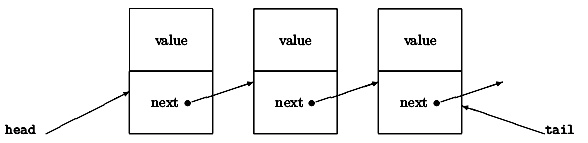
\includegraphics[scale=0.5]{linkedlist.png}
\caption{Basic illustration of a linked list}
\end{figure}

A series of \red{nodes} where each one points to the next one in memory, and
each \red{node} contains a piece of data

\medskip

Linked lists can be made as long as we want without \red{declaring} an initial size first

\end{frame}
%=========================================
\begin{frame}[fragile]
\frametitle{Linked List}
Each \red{node} in the linked lists contains data (such as an int, string, etc.) as well as a red{pointer} to the
next \red{node}of the same type

\medskip

We will build a linked list of integers.

\medskip

In order to keep track of these two elements, we create a \verb|struct| which we call \verb|Item|

\begin{block}{Example:{Every \texttt{item} has an \texttt{int} value and a pointer to next element}}

\begin{verbatim}
struct Item{
    int value;
    Item *next;
    Item (int val, Item *n){ 
        value = val; next = n; 
    }
}
\end{verbatim}

\end{block}

\end{frame}
%=========================================
\begin{frame}[fragile]
\frametitle{Linked List: Example}
The function \verb|Item| we declare inside the \verb|struct| is used to make initialization easy

\begin{block}

\begin{verbatim}
Item* p = new Item (5, NULL);
\end{verbatim}

\end{block}

instead of 

\begin{block}

\begin{verbatim}
Item *p = new Item; 
p->value= 5; 
p->next = NULL;
\end{verbatim}

\end{block}

To access the first element of the \red{list}, we 
need a \red{head} pointer to the first Item

\medskip

If we \red{lose track} of this, the 
rest of the list can no longer be \red{accessed}

\end{frame}
%=========================================
\begin{frame}[fragile]
\frametitle{Linked list operations}
Unlike arrays link list do not provide functionality to directly
access its element

\medskip

The important operations that we like the link list to support are:
\begin{enumerate}
\item to be able to add elements to our list
\item to be able to remove elements from our list
\item to be able to traverse the entire list
\end{enumerate} 

\end{frame}
%=========================================
%=========================================

\section{Abstract Data Types}
%=========================================
\section{References}
%=========================================
\begin{frame}
\frametitle{References}
\footnotesize{
\begin{thebibliography}{99} % Beamer does not support BibTeX so references must be inserted manually as below
\bibitem[tp, 2017]{p1} C++ Overview (2017)
\newblock Website
\newblock \url{https://www.tutorialspoint.com}
\end{thebibliography}
}
\end{frame}

%------------------------------------------------

\begin{frame}
\Huge{\centerline{The End}}
\end{frame}

%----------------------------------------------------------------------------------------

\end{document} 